\SetWatermarkText{Theodore Tubbs}
\DeclareGraphicsExtensions{.pdf,.png,.jpg}
\SetWatermarkScale{.75}
\doublespacing
\section{Introduction}
\paragraph{}
The social stigmatism of ``Men/Women in Drag'' or the more ``politically
correct'' term, crossdressing is prevalent in not only modern society, but in
the past as well. Gender identity and gender roles have always been seen as
bipolar opposites in society, but we live in an age where we know this is not
true. The current societal gender roles and identity rules jump to conclusion
and assume a system of binary gender, discriminating against those who do not
fit into the societal norms.
\par

\section{Body}
\subsection{The Status Quo: Men}
\paragraph{}
In today's society it is often thought that males are supposed to adhere to
certain ``unspoken'' societal guidelines, and if one steps out of these
guidelines it is often frowned upon. While I say ``unspoken'' societal guideline
Masculinity is barely that. A brutal ancient code of standards of, ``how to be a
man'' Masculinity is an old-fashioned well-intended misguided approach on ``how
to raise johnny properly''.
\par

\subsubsection{Argument: Against the Status Quo}
\paragraph{}
To sick to a ``status quo'' set in times much different then our own today is
nothing but a fallacy, it is clear times have changed since the days where ``men
were men, and women were women''. So why do males keep adhering to outdated
concepts that society pushes on them? It is sadly a cause that poisons itself
form the inside out, though it has external pressures as well, don't think men
are the only influence on how other men dress. The female can be just as guilty
and bigoted as her male counterpart.
\par

\paragraph{Males}
Pressuring other males to conform to a societal standard is
nothing new, for hundreds if not thousands of years ``man'' has formed rules of
how to act in society. As many civilizations were patriarchal (though there have
been and were matriarchal societies as well) it is only ``common sense'' that ``
man'' should be the one to create the rules, thusly leading to the societal
status quo of how ``man'' should act.
\par

\subparagraph{Example one}
``I actually had issues all my life around my gender identity. As a child, I
wanted things a neighbor friend used to tell me were incorrect; I wanted to play
house and wanted to have a baby when I got older.'' \cite[p.~478]{MOT} . In this
example this person is merely named ``MS. L'', as you might have guessed ``MS. L
'' is a \textit{heterosexual} male adult who even early on in life knew his
``real'' gender wasn't male and perused crossdressing as a way to alleviate the
feelings he had when ``MS. L'' identified as a heterosexual male. As you would
also assume ``MS. L'' has gone through hormone therapy, surgeries and support
groups to become a ``female'' now.
\par

\subparagraph{Example two}
``I started with spironolactone without estrogen. The effect for me was a lack
of drive or energy. But when the estrogen started, it was wonderful; it just
felt like it was more and more me. I’m extremely happy. A lot of wonderful
feelings and changes accompany it, not just on the physical level, but
emotionally and mentally.'' \cite[p.~479]{MOT} . ``MS. L'' pursued her desire to
identify herself as a heterosexual female and ended up improving her outlook and
feeling upon life, instead of conforming to the male stereotype and not being
happy with herself. Though as you'll see in the next example everything doesn't
go exactly smoothly.
\par

\paragraph{Example three}
``The first people I told were close friends; they were very understanding.
There has been some rejection and loss, but the acceptance and the strengthening
of relationships, certainly with women, has been tremendous. My social circle
has increased. Within my own family, it has been a hard aspect for them to
accept.'' \cite[p.~478-479]{MOT} . Of course straying from the ``status quo''
has its negatives, in this case the loss of social bonds that ``MS. L'' once had
with past friends and family. Though ``MS. L'' has accepted this in an
understanding and healthy manor.
\par

\subparagraph{In conclusion}
straying from the ``status quo'' has its pros and cons but in the end it's
better to live a happy life of fulfillment then one of emptiness and desire.
Though this argument is not one-sided and is in fact multifaceted.
Transgenderism, crossdressing, and the life are very tough and touchy topics for
people to deal with right now, one can only hope it won't be this way forever
and as a race humans can move on.
\par

\subsubsection{Argument: For the Status Quo}

\subparagraph{Example one}
``A reader writes: ``I am a straight male and consider myself fairly liberal.
One of my best friends is openly gay and I have never felt uncomfortable around
him. Yet the thought of being around a transgender person is extremely
uncomfortable to me and I don’t exactly know why.'' '' \cite[p.~1]{WDTMU} .
While this isn't an example of aggressive unacceptance of people who crossdress
or are transgendered, rather a more innocent ignorant case of confusion, this
straight male, for examples purposes let us call him ``John'', while ``John''
doesn't mean to offend any transexual/crossdressing individuals his mental
concepts of gender are being challenged and this is only a harmless reaction to
``John'' being confused. Most likely ``John'' can seek knowledge and a solution,
and possibly feel comfortable around transgendered/crossdressing individuals.
Crossdressing and Transgenderedism doesn't follow the ``status quos'' society
has in place, so it's a perfectly normal reaction for people to at first not
feel comfortable about it. But over time people should grow to accept it.
\par

\subparagraph{Example two}
``Western culture has established very specific and very strict parameters for
being a ``man'' and being a ``woman.'' And as much privilege as straight men
have in this culture, you are constantly walking an extremely narrow tightrope
in order to stay within those parameters and maintain your acceptable standing
as a straight man. \\~\\ Masculinity, as our culture defines it, is highly
valued, and as a straight man, you are expected to possess it---in exactly the
way it is defined. You are not only supposed to possess it, but you are supposed
to value it at least as much as the culture does.'' \cite[p.~1]{WDTMU} . In this
quote of the letter we see the author is explaining to ``John'' why he may or
does feel uncomfortable around transgendered/crossdressing individuals.
\par

\subparagraph{Example three}
``If you fail to do so, you are somehow considered ``deficient'' as a man---you
are not ``manly'' enough, you are not ``masculine'' enough. Something is wrong
with you if you don’t value traditional, culturally defined masculinity and do
everything you can to cultivate it, maintain it, and celebrate it.''
\cite[p.~1]{WDTMU} . This is a more ``aggressive'' example the author gives
``John'' on why society isn't normally accepting of individuals who don't follow
the ``status quo''. As we see in the quote if the status quo is not maintained
one is ``not manly enough'' and ultimately falls into social ostracization.

\subsection{The Status Quo: Women}
\paragraph{}
Unlike males, women are given more of a freedom in their variety of clothing.
For example, they can wear clothing of either gender, ``females'', or ``male''
clothing typically without being judged. Not to say judgment of women wearing
men's clothing doesn't exist. To Clarify In this section of the essay I will
define ``crosssdressing'' for women as ``a women wearing any article of which
is typically thought to be ``males'' clothing, e.g. t-shirts, jeans, shirts,
etc, etc. ''
\par

\subsubsection{Argument: Against the Status Quo}
\paragraph{}
Not to contradict myself or sound like a hypocrite, \textit{but} even for women
there are these ``unspoken'' guidelines on how to wear or what to wear in terms
of clothing, which in my opinion is mostly influenced by the enviorment around
them(no duh sherlock), e.g. TV shows, Movies, Social Media, Texts, Pictures,
ads, etc, etc.
\par

\subparagraph{Example one}
``After a few weeks ``Kazik'' was reassigned to an artillery unit, serving there
for six months, and seeing action during the Brusilov Offensive. She also
learned to ride a horse, and served in a signals platoon. After returning to
Warsaw in 1917 following the Oath crisis Gertz joined the women's branch of the
clandestine Polska Organizacja Wojskowa (``Polish Military Organization'')''
\cite{TWBS}. This is a quote from ``Wanda Gertz - the woman who was born a
soldier'' in which Wanda Gertz a woman crossdresses to serve in the Polish
military. The reason behind her crossdressing was the fact that at the
time(late 19th century to early 20th century) girls could only become private in
the Polish military. Through her heroics earned many metals, and she later went
on to lead the women's sabotage unit for the Home Army among other things. If
Wanda had simply stuck to the ``status quo'' and not disguised herself as a man
she wouldn't of helped her country with the war effort in the valiant way she
did.
\par

\newpage
\subparagraph{Example two}
``As Smirnowa recounted to the newspapers, the girls left their Moscow school
without informing anyone on the eighth day of mobilization---i.e., at the end of
July 1914. They traveled to Lviv where they dressed as men and enlisted in the
army undetected. When the first bombs fell on their position, they cried out,
as did many of the men. One girl, Zina Morozov, was killed in the Carpathians
when a bomb fell at her feet. She was buried by her friends. Two other girls
were subsequently wounded. After Smirnowa was wounded, her gender was
discovered.'' \cite[p.~365-67]{YGFRF}. Again we see another example of female
heroism because Smirnowa(and her friends) stepped outside of the ``status quo''.
\par

\subparagraph{}
In fact the men became quite accepting of the girls in the regiment.
````The girls almost forgot their past,they hardly responded to their feminine
names, for each of them had received a masculine surname, and completely mingled
with the men. The soldiers guarded the girls and observed each other's conduct.
'''' \cite[p.~366]{YGFRF}. In this example we see the acceptance of the
schoolgirls and their personality changes. Proving that even in times we
wouldn't think accepting of such actions, there were people who understood the
choices they made.
\par

\subparagraph{Example three}
``While in hiding, Belinfante learned of the arrests and executions of the other
CKC members, including Arondeus. Belinfante disguised herself as a man and lived
with friends for 3 months  before being traced by the Nazis''
\cite[t.~00:28:40-00:39:00]{BIWG}. In this situation crossdressing was a life or
death situation of disguises. To break the rules of society meant the ultimate
safety of her life.
\par

\subsubsection{Argument: For the Status Quo}

\paragraph{}
In this section we take a look at the possible drawbacks of the corssdressing of
women, the ``cons'' of breaking ``status quo''.

\subparagraph{Example one}
We go back to the story of Zoya Smirnowa. ``On being discharged she again
proceeded to the positions, endeavoring to find her regiment, but on reach the
familiar trenches she could no longer find a single regimental comrade, nor a
single fellow-volunteer; they had all gone to another front, and in the trenches
sat absolute strangers. The girl lost her presence of mind, and for the first
time during the entire campaign began to weep...'' \cite[p.~367]{YGFRF} We see
here the damaging psychological effects of war, subsequently causing Smirnowa to
have what could be assumed as a PTSD episode. Though her intentions be heroic,
consequences for her mental state of mind were grave.
\par

\subparagraph{Example two}
````During one of the Carpathian engagements at night, one of the twelve
friends, the sixteen-year-old Zina Morozov, was killed outright by a shell.
It struck immediately at her feet, and the entire small body of the girl was
torn into fragments.'''' \cite[p.~366]{YGFRF}. You could say in this instance if
the girl or girls had just stayed home, not crossdressed, and joined the
military lives could have been spared.
\par

\subparagraph{Example three}
````Was it terrible?'' an officer asked Zoya. ``Were you afraid?'' ''I should
say so! who wouldn't be afraid? When for the first time they began to fire with
their heavy guns, several of us couldn't stand it and begin to cry out'' ''what
did you cry out?'' ''We began to call `Mamma' '' \cite[p.~366]{YGFRF}. The
Traumatic effects of PTSD(Specifically ShellShock most likely) are prevalent
again sadly.
\par

\subsection{The Societal Stigma}
\subsubsection{The Current State.}
\paragraph{}
the diagram below illustrates the assumed binary gender roles of society. Yet in
modern society we know that gender is no longer a binary thing.

\begin{figure}[h!]
	\centering{}
		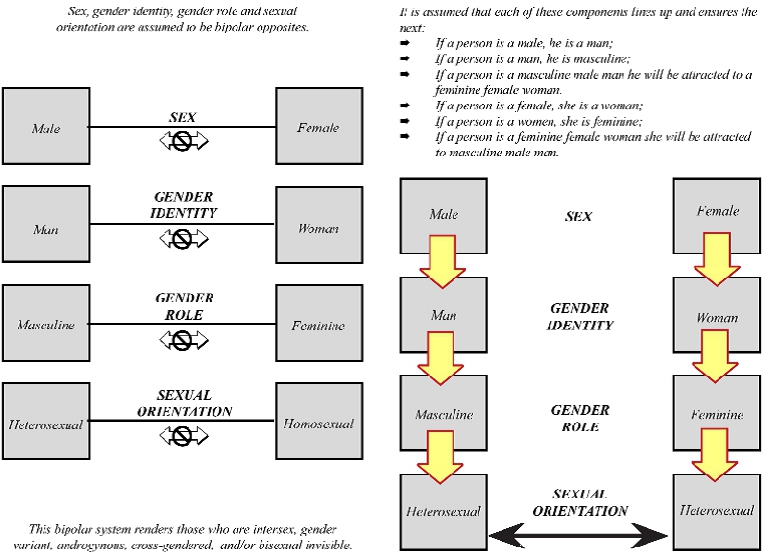
\includegraphics[scale=0.6]{figures/gender-roles}
	\caption{Typical gender roles in modern society.\cite[figure 3.3-3.4]{UDGIE}}
\end{figure}


\newpage
\printbibliography
